\chapter{Principali problemi di elaborazione digitale}

%\section{Principali problemi di elaborazione digitale}

Al giorno d'oggi i computer permettono una vasta gamma di elaborazioni digitali, ce ne sono alcuni, più semplici ma di notevole interesse, ormai già perfezionati ed altri che sono ancora oggetto di studio.

\section{Rotazioni, riflessioni,etc}
Le più semplici in assoluto riguardano "movimenti rigidi" come la traslazione o la rotazione, o anche omeomorfismi come la riflessione. Questi sono molto utili per introdurre i primi concetti matematici, come l'impiego di matrici.\\
Definiamo una matrice di trasformazione che moltiplicata per un vettore di coordinate ci restituisca un altro vettore di coordinate. Questo vuol dire che quel punto va spostato dalle coordinate in cui si trovava a quelle appena calcolate. Ad esempio:

$$
{\begin{bmatrix}
-1&0&0\\
0&1&0\\
0&0&1
\end{bmatrix}}
$$

\noindent
\`E una matrice di riflessione lungo l'asse verticale, infatti: 

$$
{\begin{bmatrix}
-1&0&0\\
0&1&0\\
0&0&1
\end{bmatrix}}
\begin{bmatrix}
x\\y\\1
\end{bmatrix}
=
\begin{bmatrix}
-x&y&1
\end{bmatrix}
$$	

\vspace{1em} \noindent
Cioè ogni punto rimane alla stessa quota ma cambia la propria x con -x, che è esattamente ciò che intendiamo per riflessione lungo l'asse verticale.

\newpage \noindent 
Altri esempi possono essere:

\begin{align*}
&\begin{bmatrix}
1&0&0\\
0&-1&0\\
0&0&1
\end{bmatrix}&~&
\text{Riflessione lungo l'asse orizzontale}\\
\\
&\begin{bmatrix}
2&0&0\\
0&1.5&0\\
0&0&1
\end{bmatrix}&~&
\text{Scalamento}\\
\\
&\begin{bmatrix}
\cos(\theta )&\sin(\theta )&0\\
-\sin(\theta )&\cos(\theta )&0\\
0&0&1
\end{bmatrix}&~&
\text{Rotazione di un angolo theta}\\
\end{align*}



\section{Cambio prospettiva}
Una delle trasformazioni più semplici è quella del cambio prospettiva. Una volta compresa questa trasformazione si è fatto anche un primo passo per parlare di warping, di cui parleremo più avanti.

\vspace{1em} \noindent
Supponiamo di avere la foto di un documento poggiato su una scrivania e di volerla migliorare in modo da estrarne solo il documento e che i suoi bordi concidano quindi con i bordi dell'immagine.

\vspace{1em} \noindent
In genere la cosa più semplice ed affidabile è quella di far scegliere i 4 angoli del documento ad un utente. Volendo automatizzare il processo possiamo però scegliere un'altra strada: ossia estrarre i bordi dell'immagine e cercare tra questi quelli che formano un trapezio, presumibilmente quello sarà il documento.

\vspace{1em} \noindent
Ottenuti i 4 angoli, calcoliamo la lunghezza e la larghezza della nostra nuova immagine. Per fare ciò iniziamo con il calcolare la lunghezza dei 4 lati, questi li otterremo banalmente con il teorema di Pitagora. A questo punto prendiamo i lati a due a due non adiacenti, cioè che non hanno vertici in comune e ne confrontiamo le lunghezze.\\
Per ogni coppia prendiamo la lunghezza maggiore (si può anche usare quella minore ma non dilunghiamoci su questa scelta).

\vspace{1em} \noindent
Ora siamo in grado di calcolare la matrice di trasformazione. Essa sarà del tipo:

\begin{align*}
&\begin{bmatrix}
a_1&a_2&b_1\\
a_3&a_4&b_2\\
c_1&c_2&1
\end{bmatrix}
\text{ dove }
\begin{bmatrix}
a_1&a_2\\
a_3&a_4
\end{bmatrix}
\text{ definisce rotazione e scalamento, } 
\begin{bmatrix}
b_1\\
b_2
\end{bmatrix}
\text{ è un vettore di}\\
&\text{traslazione e} 
\newline
\begin{bmatrix}
c_1&c_2
\end{bmatrix}
\text{ è un vettore di proiezione (che è nullo se il riquadro iniziale e quello}\\
&\text{finale coincidono).}\\
\end{align*}

\vspace{-3em}

\begin{align*}
&\text{L'intento è che moltiplicando tale matrice per il vettore  }
\begin{bmatrix}
\text{coordinata x}\\
\text{coordinata y}\\
1
\end{bmatrix}
\text{ otterremo il vettore}\\
&\begin{bmatrix}
\text{nuova coordinata x*k}\\
\text{nuova coordinata y*k}\\
k
\end{bmatrix}
\text{ eseguendo questa operazione per tutti i punti, costruiamo l'immagine}\\
&\text{desiderata.}
\end{align*}

\section{Morphing}
Il morphing è uno dei primi effetti digitali sviluppati dall'industria cinematografica e consiste nella trasformazione fluida, graduale e senza soluzione di continuità tra due immagini di forma diversa, che possono essere oggetti, persone, volti, paesaggi.

\vspace{1em} \noindent
Il morphing non è altro che l'uso in contemporanea di una dissolvenza incrociata e di un effetto di deformazione chiamato warping (termine inglese che significa appunto deformazione).

\vspace{1em} \noindent
Per operare il warping si definiscono sull'immagine di partenza dei "punti chiave" che possono essere uniti tra di loro con delle linee e si definiscono sull'immagine di destinazione i corrispondenti punti e di conseguenza le corrispondenti linee.\\ 
\begin{figure}[htb] \centering
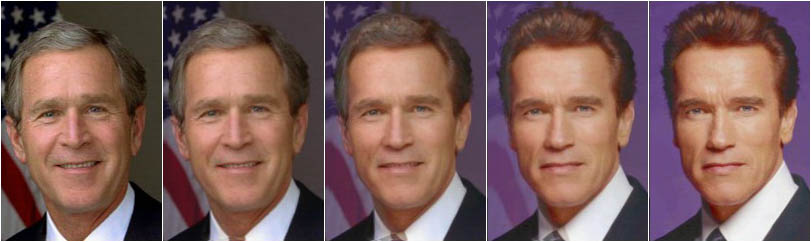
\includegraphics[scale=0.5, trim = 0 1.1cm 0 0, clip]{Pictures/Striscia_morphing.jpg}
\caption{Processo di morphing con alcuni risultati intermedi.}\label{fig:figura}
\end{figure}

\noindent
Durante la dissolvenza dall'immagine iniziale a quella finale, le immagini vengono deformate facendo in modo che ciascun punto chiave si muova lungo il percorso che porta dalla sua posizione nell'immagine di partenza alla posizione del corrispondente punto nell'immagine di arrivo.\\